
\chapter{Fundamentals of Software Performance Testing}
\label{Fundamentals of Software Performance Testing}
The usual goal of the performance testing is to ensure that the application runs reasonably fast enough to keep the attention of users, even with unexpected amount of clients using the application at the same time. But why is it so important to have the application optimized for the best speed? Simply, when your application has slow response, long load time or bad scalability, the first website which user will visit afterwards will be the web of your competitor. That is the reason why speed is currently one of the most significant performance factor of common performance problems. This chapter summarizes the fundamentals of the performance testing which includes definitions of common performance processes, issues, and metrics, based on knowledge available in \cite{Molyneaux:TAoAPT, Kurkova:Thesis:2017, DIN:PHD, ISTQB}.


\section{Performance Testing Process}
\label{Performance Testing Process}
The main goal of the performance testing is to ensure the following application attributes \cite{GAO:MEASURING}:

\begin{description}
	\setlength\itemsep{0em}
	\item \textbf{Reliability and Stability}\,---\,the ability of software to perform its functions in system environment under some system load for acceptable\footnotemark{} period of time,
	\item \textbf{Scalability}\,---\,the ability of software to behave properly under various types of system load and handle increasing amounts of workload (such as network traffic, server load, data transfer, etc.) which would need new hardware for cluster expansion,
	\item \textbf{Processing time and Speed}\,---\,the ability of software to react quickly without low response time during any acceptable system load,
	\item \textbf{Availability}\,---\,the ability of software to make all of its functions available during any acceptable system load. The ability of software, deployed in cluster, to provide all functions during node crash is called High Availability.
\end{description}

\footnotetext{During software development there is a document with Software Requirements Specification which specifies software metrics, including performance.}

Similarly to software development process, performance testing process consist of usual engineering steps ranging from requirements definition to data evaluation. These steps also includes design, implementation, and execution of performance tests with data collection. The graphical representation of the performance testing process is depicted in the Figure~\ref{fig:performace_testing_process}.

\begin{figure}[H]
  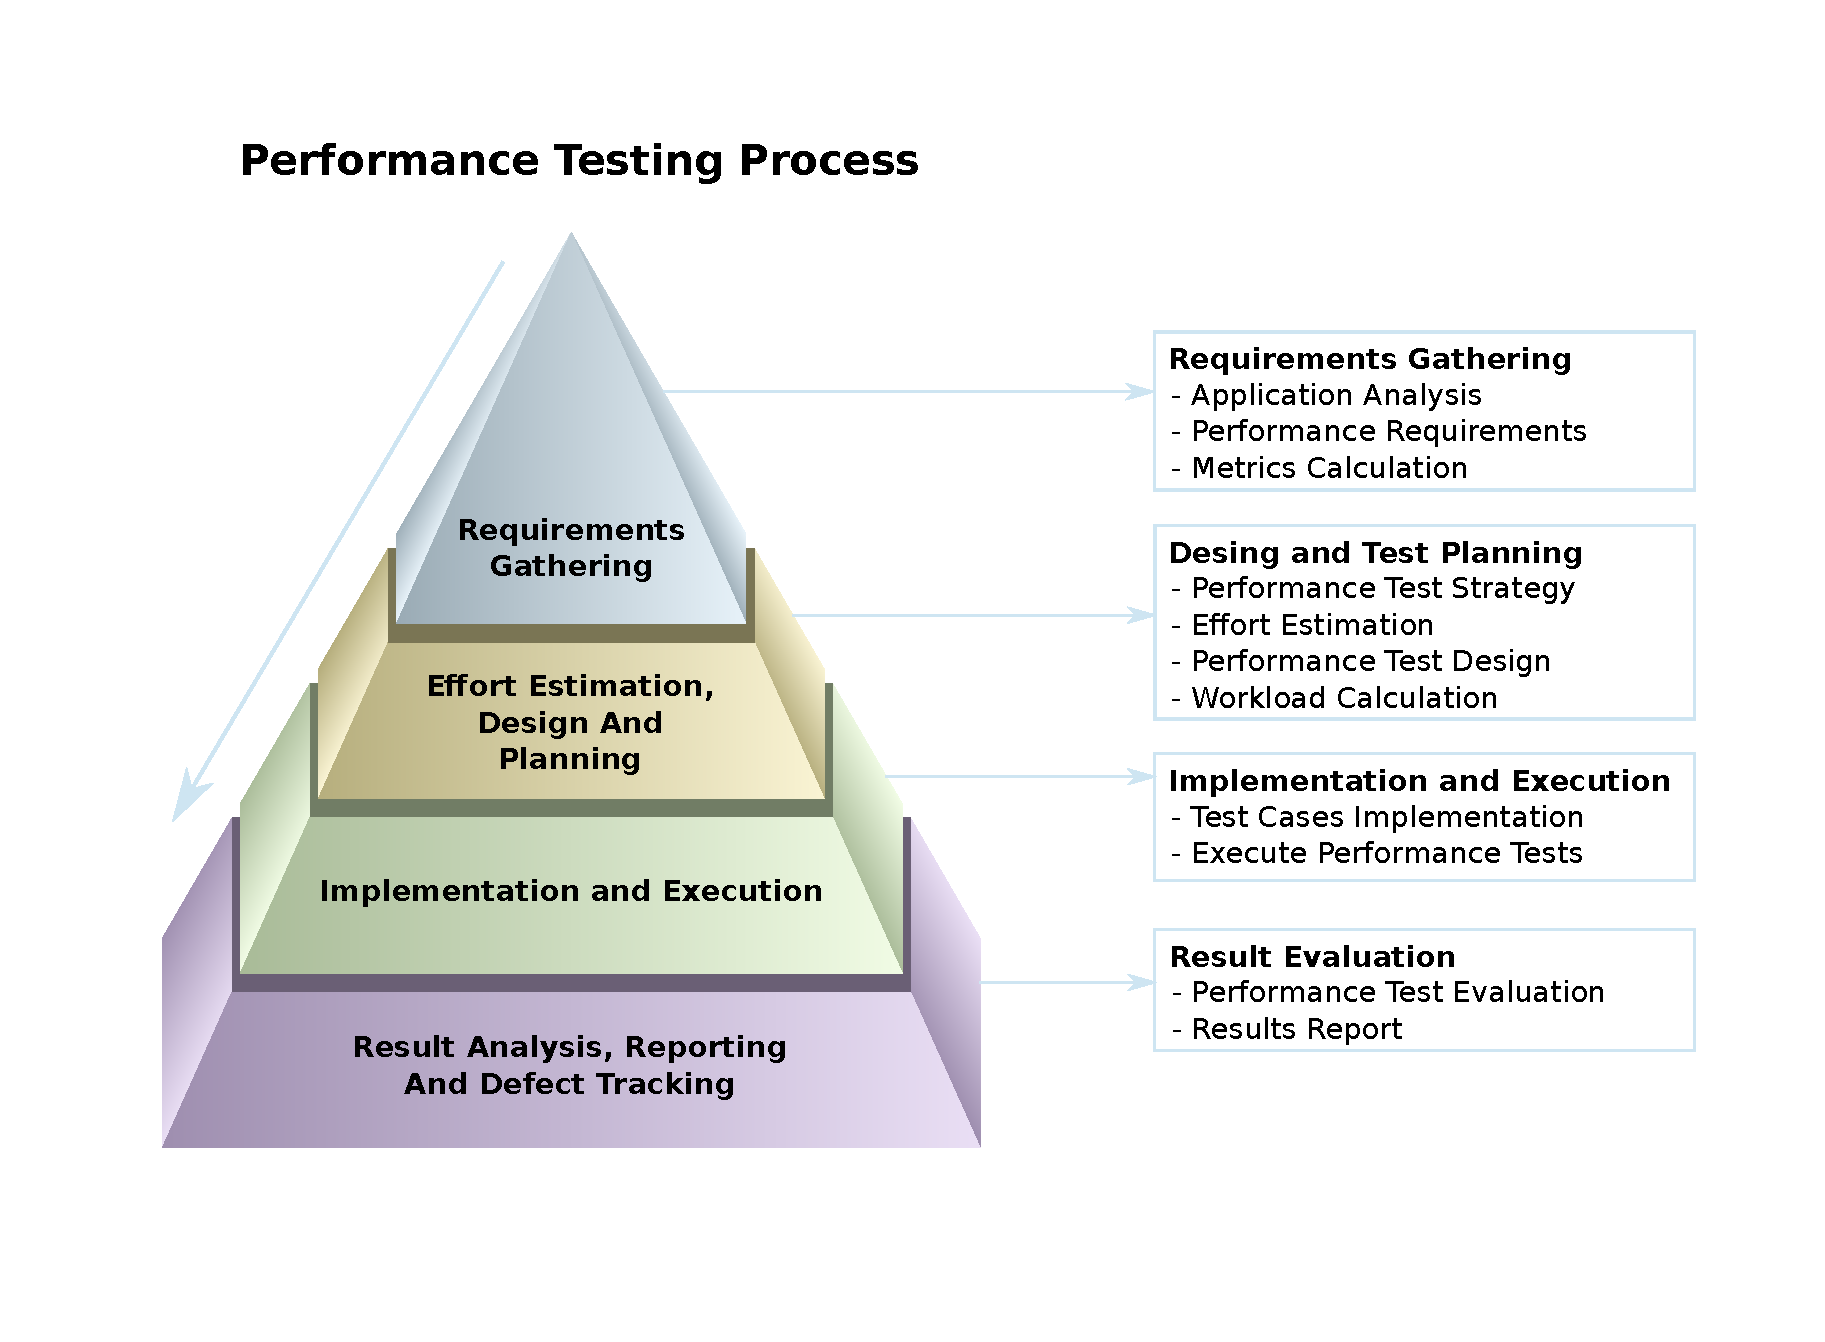
\includegraphics[width=16cm]{obrazky-figures/pyramid.pdf}
  \caption{The performance testing process with the four most important parts and theirs individual steps based on \cite{Sharma:HP}.}
  \label{fig:performace_testing_process}
\end{figure}
In the Figure \ref{fig:performace_testing_process} you can see the scheme of performance testing process where each level represent required time for each step. Lower levels refers to more time spend on that step.

The first step of performance testing process is the selection of \emph{performance requirements} for the application. In this step, testing engineer has to analyze \emph{software under test\,---\,SUT}, chose suitable performance metrics, that will model the application performance, and state performance requirements, usually with customer and project manager. The result should include answers to questions such as:

\begin{itemize}
	\setlength\itemsep{0em}
	\item How many end users will the application need to handle at release, after six~months or in one year?
	\item Where will these users be physically located, and how will they connect to the application?
	\item How many end users will be concurrently connected in average at release, after six~months and one year?
\end{itemize}

Based on answer to these studies, the engineer should be able to select important key performance indicators for performance test cases. Some of these indicators may be \emph{response time}, \emph{stability}, \emph{scalability}, or \emph{speed}. However, there is huge amount of possible indicators so it is necessary to properly analyze the whole application and also take into consideration another needs such as error rate, system resources, etc.  Result of this phase should be a~binding document with all performance requirements to be tested, and in case of detected performance degradation, such defect must be fixed w.r.t this document.

The next step is to define the \emph{performance testing strategy}, corresponding to the planning and design. It is extremely important to allocate enough time for SUT testing effectively, because, as it was mentioned in Chapter \ref{Introduction}, performance testing is not an easy task and detecting all of the possible issues of tested components is very time consuming process. Every plan should take into account the following considerations:

\begin{description}
	\setlength\itemsep{0em}
	\item \textbf{Prepare the test environment}\,---\,this step includes choosing the right hardware for the testing, then installing the necessary software for running load injectors, tested components, etc., and preparing other equipment depending on the application purpose such as routers, switches, mobile devices, etc.
	\item \textbf{Provide sufficient workload injectors}\,---\,preparing the workload injectors may take few days; we usually require few workstations or servers to simulate the real traffic.
	\item \textbf{Identify and implement use cases}\,---\,this includes identification of important parts of the system which may have an impact on performance; time needed for each use case may be different because some use cases can be simple such as navigating to a web application home page, but some may be complex such as filtering specific communication.
	\item \textbf{Instrument the test environment}\,---\,install and configure the monitoring software on the test environment.
	\item \textbf{Deal with detected problems}\,---\,tests can detect significant performance issues, but their investigation and the actual fixes may take a long time. After the fix the retest of issue is needed.
\end{description}

While this process seems trivial, the opposite is true, especially in cases of network applications. Most of the performance issues manifest with big workloads or high number of users, e.g. when million users are sending requests to the network device at the same time it can lead to an unacceptable device crash. Workload injectors are designated to simulate real user activity, and allows automatic analysis of performance behavior for tested application or device. Depending on the used technology, there can be a limit on the number of virtual users that can be generated by a single injector. These automated workload injectors are necessary for effective performance testing.

After describing the plan we implement and execute proposed test cases. Environment and workload injectors are ready for the execution, so the last step before the testing itself is the implementation of tests. Thanks to the careful planing, engineers should have enough time to implement test cases with reference to proposed design.

The final step of the performance testing process is evaluation of the results. Output of this step is usually technical report with all selected performance key indicators, used workload and Collected Data Format for each test case. Then follows the data evaluation with thorough analysis of degradation localization. Additionally, the report usually contains syntactical graphs which display performance metrics along the duration of test execution.

\section{Performance Issues}
\label{Performance Issues}
A~\emph{performance issue} is a common label for an unexpected application or device behavior which affects its performance. Usually, those issues are hard to detect because they manifest only under certain circumstances such as high load or long application run time. In the network applications there are several particular issues that are more frequently occurring  than others. In the following, we~will describe selected issues in more details.

\subsection*{Performance Degradation}
\label{Performance Degradation}
An unclean code usually leads to inefficient algorithms, application deadlocks, or memory leaks, which all can eventually cause a performance degradation. The problem is that these issues are usually detected only during the long run time of application or inability of an application to handle high load. For this kind of issues there is a performance testing method called the \emph{endurance testing} \cite{BUCH:4TYPES, Manzor:APTB} which is described in Section \ref{Endurance Testing}. The endurance test is intended to identify problems that may appear only after the long period of the application run-time\footnotemark{}, hence its necessary to run this type of tests during the application development. The network applications usually need to be available for 24 hours per day. The duration of a endurance test should have some correlation to the operational mode of the system under test. Following scenarios may represent performance issues detectable by endurance tests:

\begin{itemize}
	\setlength\itemsep{0em}
	\item a constant degradation in response time, when the system is run over the time,
	\item any degradation in system resources that are not apparent during short runs, but will surface during the long run time such as free disk space, or memory consumption,
	\item a periodical process that may affect the performance of the system, but can be detected only during the long run time such as a backup process, exporting of data to a 3rd party system, etc.,
	\item a development of new features for already existing components.
\end{itemize}

\footnotetext{Soak Test\,---\,refer to HW testing method during where engineers soak device into water and check for bubble leaks.}

\subsection*{Response Time}
\label{Response Time 1}
Response time represents how long it takes for system to accept, evaluate, and respond to the user for his request e.g. HTTP request for the particular website. Different actions and requests can have significantly different response time and with that provide different load on the system. For example retrieving document from a web-server by its ID is considerably faster than searching for the same document by keywords. Response time is mostly measured during the \emph{load test} \cite{Manzor:APTB} of the application. Well designed test should consider different types of load on the system, various kind of requests, and different number of connected end-users at the same time. For user based systems we usually consider three thresholds for the response time values:

\begin{description}
	\setlength\itemsep{0em}
	\item \textbf{0.1 second}\,---\,this represent an ideal response time for the application, because user feels that system is reacting instantly and does not notice any interruptions.
	\item \textbf{1 second}\,---\,this is the highest acceptable response time when user still does not feel any interruptions, but can feel a little delay; this still represent no bad impact on the user experience.
	\item \textbf{10 seconds}\,---\,this is the limit after which response time become unacceptable and user will probably stop using the application.
\end{description}

However response time thresholds for non-human interactive system are more strict. They can range in milliseconds or less.


\subsection*{Traffic Spikes}
As a \emph{traffic spike} \cite{Kurkova:Thesis:2017, AMC:SPIKES} we can understand the sudden surge in demand from users. Typically manifesting by doubling or multiplying of traffic level in a short period of time. In a real network, spikes are result of high workload, e.g. caused by higher amount of users trying to concurrently use the service over the network. For example we can experience a sudden traffic spike in response time after publishing new popular viral content on video servers, start of sales events, reservation of limited amount tickets or subject registration at university. Scheduled automatic backup or system upgrade for whole company during early morning hours can also cause traffic spikes.

Traffic spikes can lead to the inappropriate system behavior such as \emph{long response time}, \emph{bad throughput}, and \emph{limited concurrency}. To prevent the impact of traffic spikes on system performance, it is necessary to do a sophisticated infrastructure monitoring and network load analysis, in order to distinguish between normal traffic and an attack on the system. Suitable methods for testing of spikes is one of variant of \emph{stress testing} \cite{Manzor:APTB} and it is described in Section \ref{Types of Performance Testing} in more details. Network system should offer load balancing, thus it should be able to redirect traffic to another node with same service in case of high load which can cause performance issues due inappropriate resource usage.

\begin{figure}[H]
  \centering
  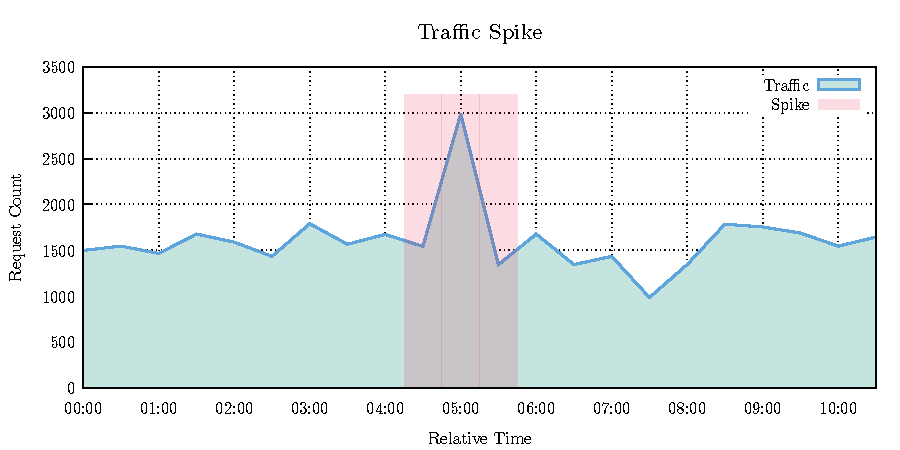
\includegraphics[width=14cm]{obrazky-figures/traffic_spike.pdf}
  \caption{The graph shows amount of concurrent sessions depending on time. During to network traffic monitoring we can see the traffic spike occurring after five hours from test start.}
  \label{fig:spikes}
\end{figure}

\section{Types of Performance Testing}
\label{Types of Performance Testing}
% % http://www.wmrichards.com/high_performance_messaging.pdf 2017/10/18

For performance testing there are many types of suitable test methods. Which test you should use is determined by the nature of the system, testing requirements or how much time we have left for the performance testing. The following terms are generally well known and used in practice and each of them characterizes a category or suite of the tests:
\begin{itemize}
	\item \textbf{Testing methods}\,---\,load testing, stress testing, endurance testing,
	\item \textbf{Testing approaches}\,---\,smoke testing, regression testing, benchmark testing.
\end{itemize}

Their description is based on the knowledge available in \cite{TuPo:TESTS, BUCH:4TYPES, Molyneaux:TAoAPT, ISTQB}.

\subsection*{Load Testing}
Finding the maximal load is a testing method which studies how the system behaves during different types of workload within acceptable time range. Basically, it simulates the real-world load. During the load test we mainly focus on response time metric of the system for requests. Requests are generated by users or another systems communicating with the SUT. The main goal is to determine if the system can handle required workload according to performance requirements. Load test is designed to measure the response time of system transactions under normal or peak workload. When the response time of the system dramatically increases or becomes unstable, we conclude that system has reached its maximum operating capacity. After the successful testing, we should mark the workload requirements as fulfilling or analyze the Collected Data Format and report issues to the developers. In the Figure \ref{fig:load_test} you can see the graph of load test showing workload of raising requests to the web server at the same time where the system response time does not exceed 3.5 seconds.

\begin{figure}[H]
  \centering
  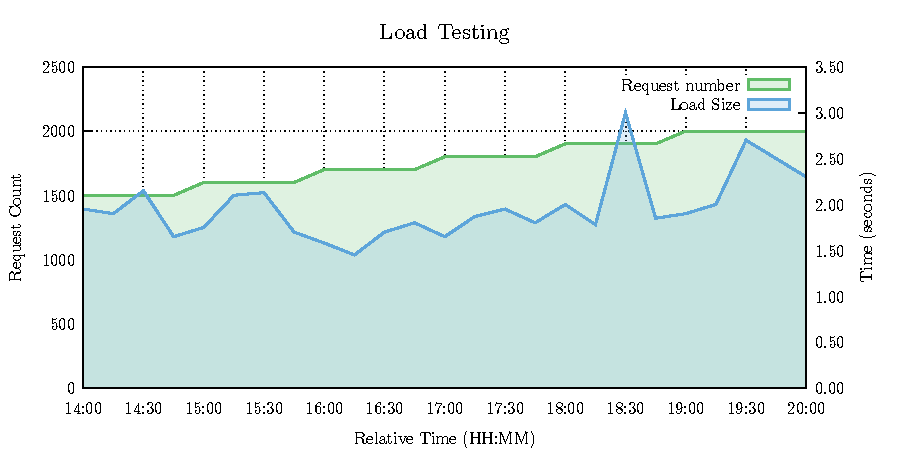
\includegraphics[width=15cm]{obrazky-figures/load_testing.pdf}
  \caption{The response time of the system during the load testing depended on requests per second.}
  \label{fig:load_test}
\end{figure}

The following list shows common scenarios for load testing:
\begin{itemize}
	\setlength\itemsep{0em}
	\item The system interacting with multiple users at same time.
	\item The system tracking communication and analyzing it.
	\item Web services and information systems.
\end{itemize}
Typical system issues covered by the load testing:
\begin{itemize}
	\setlength\itemsep{0em}
	\item Concurrent users connections can eventually result into the slow response time or system crash.
	\item Network systems without redundancy connections can shutdown the whole network under normal defined workload.
	\item Data availability during multiple sessions to data server.
	\item Connection rejection (timeout).
\end{itemize}

\subsection*{Stress Testing}
\label{Stress Testing}
Stress testing is the specific type of load testing, where we do not measure the normal workload, but focus on unexpected workloads or traffic spikes. The main purpose is to study how the system behaves in extreme conditions such as an enormous number of concurrent requests, using a server with much less memory or a weaker CPU, and analyze the system performance threshold. Its very useful to know performance threshold in order to know the difference between performance under normal workload and performance threshold. The following enumeration lists common stress test scenarios:
\begin{itemize}
	\setlength\itemsep{0em}
	\item Monitoring the system behavior with over maximum of users logged in at the same time.
	\item All user performing critical operations at the same time.
	\item All users accessing the same file at the same time.
	\item Hardware issues such as having a server in a cluster down.
\end{itemize}
Typical issues, which are covered by stress testing are as follows:
\begin{itemize}
	\setlength\itemsep{0em}
	\item A~sudden performance degradation.
	\item System will recover after the stress test (system is operational after test).
	\item System does not crash during stress test.
	\item All subsystems such as database, load balancer, etc. remains operational.
\end{itemize}

When engineers finish stress testing and finds the limits of the system, they also can test the system recovery after a crash during finding of the system limits.

In the Figure \ref{fig:stress_test} we show recorded stress testing with a raising load and response time. Everything is fine until the amount of requests exceed 3,000 requests per second. With higher load there comes performance issues which leads to unexpected rise of the response time.

\begin{figure}[H]
  \centering
  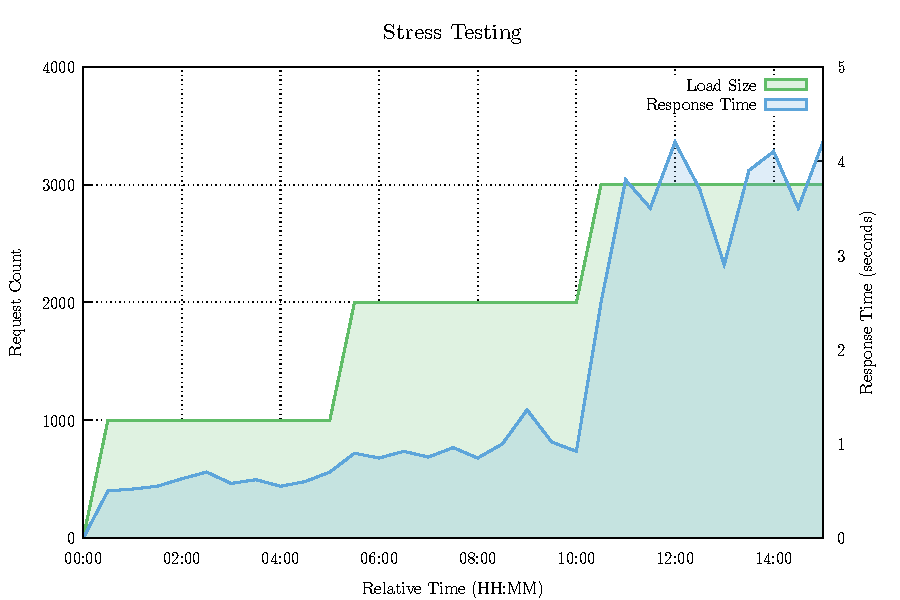
\includegraphics[width=15cm]{obrazky-figures/stress_testing.pdf}
  \caption{Stress testing diagram capturing dependency of response time on amount of requests.}
  \label{fig:stress_test}
\end{figure}

\subsection*{Endurance Testing}
\label{Endurance Testing}
The endurance, or stability/soak testing refers to the method, that tries to identify problems, that may appear only after the extended period of time e.g. The system could seem to be stable for one week, but after some longer period, problems such as memory leaks or not enough disk space can appear. Soak tests mainly focuses on measuring the memory as a performance metric. Typical scenarios for usage of soak testing:
\begin{itemize}
	\setlength\itemsep{0em}
	\item Developed system uses multiple database connections.
	\item There is a chance for inappropriately allocated memory, or memory free.
	\item Disk space limitation for store logs or other data.
\end{itemize}

The following are common issues found by soak test:
\begin{itemize}
	\setlength\itemsep{0em}
	\item A~serious memory leaks that can eventually result into the system crash.
	\item Improperly closed database connections that could starve the system.
	\item Improperly closed connections between system layers that could stall any of the system modules.
	\item Step-wise degradation that could lead to a high response time and the system becomes inefficient.
\end{itemize}


This sort of test needs to use appropriate monitoring system to achieve the high efficiency. Problems detected by soak tests are typically manifested by gradual system slowdown in response time or as a sudden lost of system availability.

\begin{figure}[H]
  \centering
  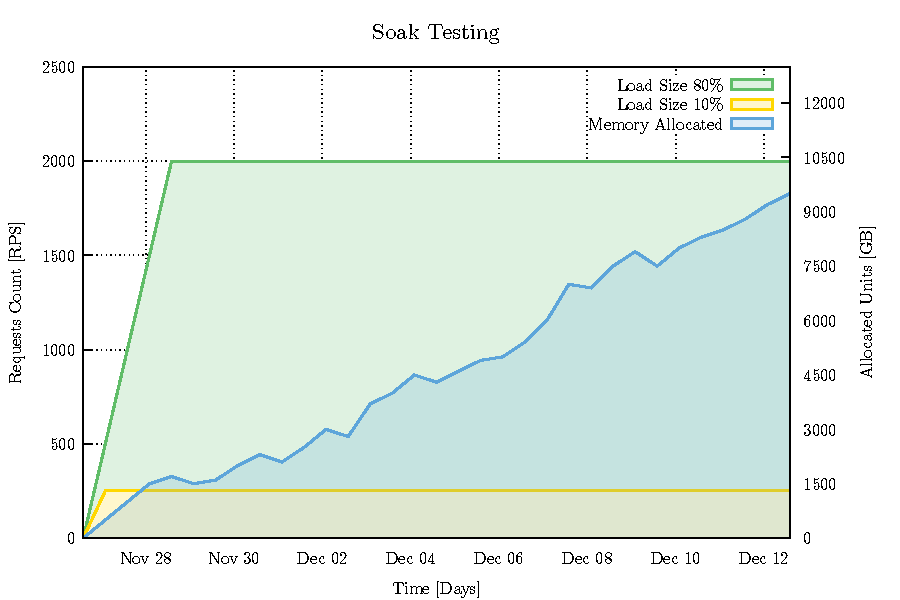
\includegraphics[width=15cm]{obrazky-figures/soak_testing.pdf}
  \caption{Soak testing with memory usage dependent on time.}
  \label{fig:soak_test}
\end{figure}

In the Figure \ref{fig:soak_test} you can see rising memory usage after period of time. The SUT can handle requests but as time goes by memory usage is too high and so the SUT will crash. This may have been caused by a memory leak or an inappropriate algorithm use.

\subsection*{Smoke Testing}
The smoke testing approach is inspired by the similar hardware technique, when engineers checks for the presence of the smoke from the device after turning the power on. Basically, its similar for software, since the main goal of smoke test is to test the basic functionality of the system and guarantee that the system is ready for the build. However, smoke tests are testing the functionality on a surface level, so they may not be enough for the deep testing of basic system functions. When smoke tests fail, the system is tagged as unstable, because it cannot ensure its basic functionality and it is not tested anymore until the smoke test pass. Smoke test are designed to uncover obvious errors which saves time, money and effort of the engineers. These tests should be used with every new build, since new features could harm previous system functionality.
The following lists show common scenarios for smoke testing:
\begin{itemize}
	\setlength\itemsep{0em}
	\item New system's build or version is ready for further testing or productilization.
\end{itemize}
Typical system issues covered by smoke testing testing:
\begin{itemize}
	\setlength\itemsep{0em}
	\item System without main functionality is useless, because test coverage of functionality is low.
	\item Main functionality resulting into a system crash.
\end{itemize}

Smoke testing is not a typical performance testing approach, but it can be used for initial load test to check if the system can be started.

%\footnotetext[\label{note1}]{Approach for test suits, where are used other methods like Load testing, Stress testing, etc.}

\subsection*{Regression Testing}
Whenever engineers develop a new feature and want to update the previous build it has to pass the \emph{regression tests}\footnote{Approach for test suits, where are used other methods like Load testing, Stress testing, etc.}\addtocounter{footnote}{-1}\addtocounter{Hfootnote}{-1} \cite{STF:REGRESSION}. Regression tests are designed to test functionality of the latest build updated with new feature. The main objective is to determine, if new feature affects already functional parts of the system. This type of tests is very important, because engineers do not always realize, which parts of the system will be indirectly affected. During the regression testing, new test cases are not created, but previous test cases are automatic re-executed and analyzed.
Typical scenarios for regression testing:
\begin{itemize}
	\setlength\itemsep{0em}
	\item New feature of system is ready for use.
\end{itemize}
Common issues covered by regression testing:
\begin{itemize}
	\setlength\itemsep{0em}
	\item New feature could adversely affect already working components of the system.
\end{itemize}

%\footnotetext{Approach for test suits, where are used other methods like Load testing, Stress testing, etc.}

\subsection*{Benchmark Testing}
The \emph{benchmark testing}\footnotemark{} is an approach, which collects performance data during the system run on different hardware machines \cite{Aho:Benchmarking}. Collected Data Format has significant value when we want smooth run of the system on an older hardware, hence we can discover performance issues under normal load. However, when the system does not run smoothly on prepared hardware, the only option is to run benchmark tests on different machines with different hardware and under different load.

\begin{itemize}
	\item Can identify minimal requirements for HW, metrics, etc.
	\item Can validate supported HW configuration.
\end{itemize}



\section{Performance Metrics}
\label{Performance Metrics}
% https://loadstorm.com/load-testing-metrics/ 2017/10/18

During the performance testing we can monitor a lot of metrics, which can have different importance based on the system's purpose. The following lists the most common metrics that are monitored during the performance testing of all applications not depending on developing language.

In the tested systems, performance metrics are collected during the long process of collection, analysis and reporting of information regarding the performance of whole the system or an individual component. This process can be different for each metric, since each metric needs different type of the system analysis.

\subsection*{The Ways to Measure}
The performance measurement process can be divided into several steps. Metrics are usually measured after a warm-up period of time after the commencement of traffic, because it takes a while for workload to stabilize. Stabilized workload is necessary for measurements because unstable workload can negatively affect the measurement results. In the Figure \ref{fig:measurements} one can see a workload phases with marked part for the actual performance testing.

\begin{figure}[H]
  \centering
  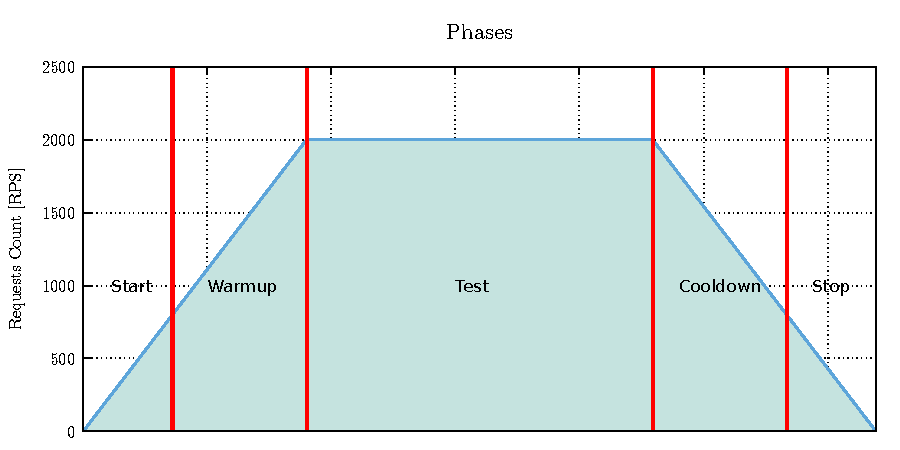
\includegraphics[width=15cm]{obrazky-figures/measure_demo.pdf}
  \caption{Load phases of performance measurement process.}
  \label{fig:measurements}
\end{figure}

Workload during testing does not have to be on the same during the whole testing. In particular, load testing finds the highest load during which the system can work properly. This limit is found by raising the load and monitoring the system as it is shown in the Figure \ref{fig:load_test}.

\subsection{Throughput}
Throughput is a metric, which refers to the number of requests per second that the system can handle. \emph{Network throughput} is the rate of successful message deliveries over a communication channel. Throughput is measured by load testing; suitable strategy for measuring throughput is to continuously raise the load until response takes longer that acceptable threshold.

\subsection{Response Time and Latency}
Slow response time as an issue was already mentioned in the Subsection \ref{Response Time 1}; response time as metric consists of two parts\,---\,\emph{latency} and \emph{service time}.

\subsubsection*{Service Time}
Service time is the time it takes the system to evaluate and send the response to the user request. In particular, when user sends a request for a web page to a server, it takes the server time to evaluate the request and send the proper response back to the user; this is the service time. Measurement can be performed easily using a stopwatch which starts when request is received and stops after the response is sent. Service time can be affected by any item which leads to a performance degradation as described in the Subsection \ref{Performance Degradation}.

\subsubsection*{Latency}
The second part of the response time is the latency \cite{Broadwell:RPT, BHATT:PERF}, which represents a delay between the sending the request on the client side and receiving it for evaluation on the server side. Hence, latency is the common problem in the network systems such as data centers, web servers, etc., because request/response needs to travel over the physical medium between the client and the server. Client and server can be located on different continents, thus the message has to travel long distance and the latency increases.

\subsubsection{Round Trip Time}
Round-trip time (RTT) is a time that it takes for a signal to be sent together with a time it takes for an acknowledgement of that signal to be received. In network, the RTT is one of the several factors that affects the signal latency. Basically, RTT depends on the distance between the sender and receiver, because that is the distance the signals must travel by.


\begin{figure}[H]
  \centering
  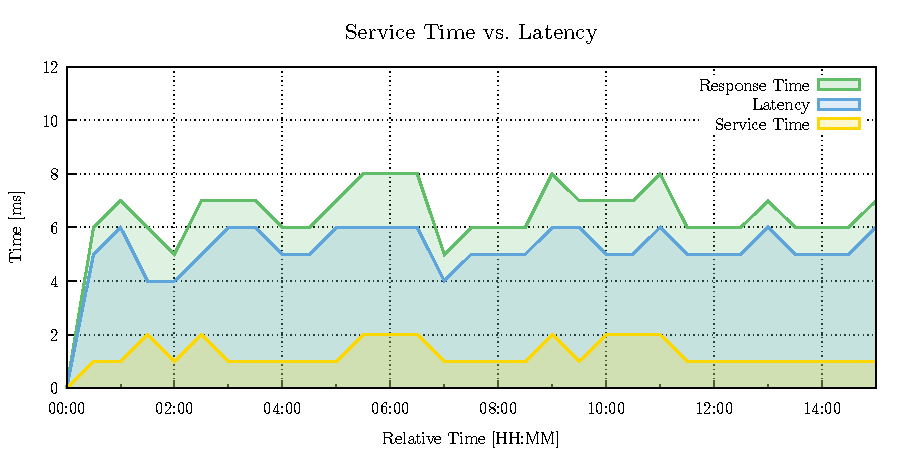
\includegraphics[width=15cm]{obrazky-figures/latency.pdf}
  \caption{Diagram capturing the difference between the latency and response time.}
  \label{fig:latency_vs_service_time}
\end{figure}

In the Figure \ref{fig:latency_vs_service_time} you can see the response time and both of it's parts: latency and service time. Service time is usually smaller than latency since latency depends on the distance. When you add service time value and latency value you will get response time at certain time.

\subsubsection*{Average and Percentile Response Time}
There are two common ways of measuring the response time \cite{Kopp:RPT}: one of them being the average (mean) response time calculated as the sum of all measured times divided by the count of users requests. While this seems trivial, in many times, the average response time does not actually reflect the real response time of the system. How is that possible? In reality, most applications have few heavy outliers such as several very slow transactions. In the Figure \ref{fig:average_percentil_1} you can see few slow transactions which drag the average of the response time to the right. This naturally leads to an inaccurate specification of response time.


\begin{figure}[H]
  \centering
  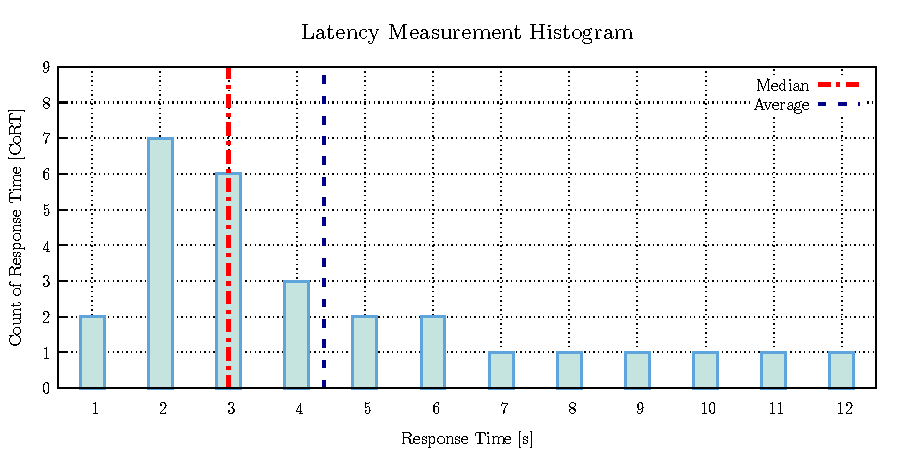
\includegraphics[width=15cm]{obrazky-figures/average_median_1.pdf}
  \caption{Transactions response time with calculated average and median of response time. The average represent inaccurate response time, which is higher than real one.}
  \label{fig:average_percentil_1}
\end{figure}

Let's look at another case, where a better solution how to determine the actual response time is the Percentile. The percentile is statistic method, which cuts measured ordered values into hundredths and then characterize the value below which a given percentage of measurements in a group of particular measurements falls. In the Figure \ref{fig:average_percentil_1} you can see the \emph{median} value, which reflects more realistic value of the system response time. Median value is same such as the 50th percentile. In this case, there is no problem, because user will expect slower response time than it has.

\begin{figure}[H]
  \centering
  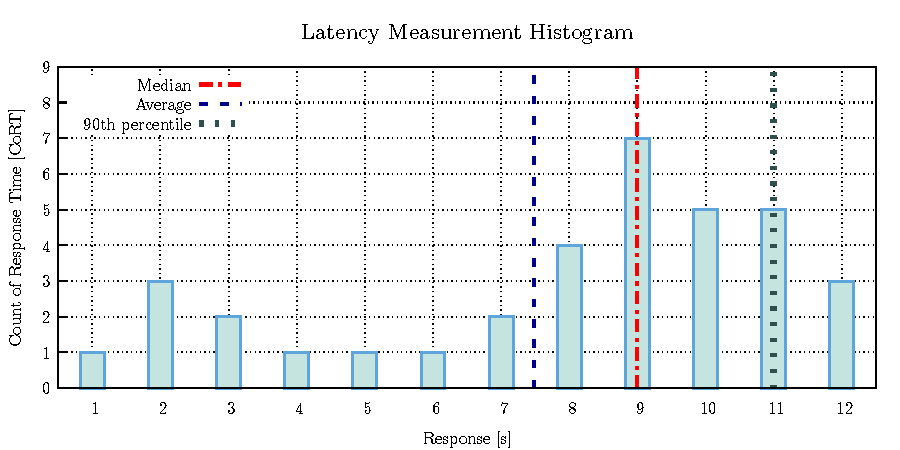
\includegraphics[width=15cm]{obrazky-figures/average_median_2.pdf}
  \caption{Transactions response time with calculated average and median of response time.}
  \label{fig:average_percentil_2}
\end{figure}

The Figure \ref{fig:average_percentil_2} shows a different situation. The average represent inaccurate response time, which says, that SUT is faster than it is in a reality. Average response time seems better than median, which reflects the expectation of faster system response time than it has. In real systems, we usually use values of the 90th percentile and the 99th percentile. 90th percentile mean, that there is only 10 \% transactions slower then marked response time. In the Figure \ref{fig:average_percentil_2}, a considerable percentage of transactions are very fast (first 50 percent), while the bulk of transactions are several times slower. Thus, the calculated percentile gets more realistic value than average response time.

\subsection{Resource Usage}
Applications running at servers with long run-time competes over a limited amount of resources available for use. Thus makes resource usage another important metric, which needs to be monitored since not enough resources could shut down the whole system. Main resources for monitoring and utilization are:

\begin{description}
	\setlength\itemsep{0em}
	\item \textbf{CPU usage}\,---\,inappropriate usage of CPU could lead to performance degradation, because low priority processes may occupy CPU ahead of the higher priority processes. CPU usage is structuring into system usage and user usage. High system usage can cause problems or bottlenecks.
	\item \textbf{Memory usage}\,---\,full consumption of memory could cause performance degradation.
	\item \textbf{Disk space}\,---\,for example when using storage disk as a database, there should be preventive measures to backup the data and free up disk space.
	\item \textbf{Operating System limits}\,---\,system's memory and CPU capabilities.
\end{description}


\subsection{Error Rate}
Error Rate is a~metric, which commonly occurs in the network systems, especially under high load. During the communication between client and server there could be error caused by another network device (router, switch, etc.) or signal disruption of the data during the transfer. The Error Rate is the mathematical calculation that produces a percentage of problem requests compared to all requests. In the ideal system, there should be a zero network errors present, however, in reality this is infeasible. This usually leads to a performance degradation and low throughput, because damaged data need to be resent.
Error rate is a~significant metric because it tells engineers how many requests failed at a particular point in time of performance testing. This metric is more evident when you can see the percentage of problem strongly increasing, hence you can detect the problem easily.
